\label{Konzept}
\chapter{Konzept}

Um sich auf die in \ref{Einleitung und Problemstellung} Einleitung und Problemstellung gennanten Zielgruppen einzulassen, hat man sich nach einiger Analyse entschieden, in einem ersten Schritt einen Chat-Bot zu programmieren, der basale Informationen vom Nutzer abfragt und den Bewerber einen Termin vereinbaren lässt. Weitere Iterationen sind nach erfolgreicher Beta-Phase möglich und ein Ausblick wird in \ref{Zusammenfassung und Ausblick} Zusammenfassung und Ausblick gegeben. Die Recherche ergibt ein Zweistufenmodell nach dem in einem ersten Schritt die Telegram Bot API genutzt wird, um einen Proof of Concept zu erstellen und eine geskriptete Variante des Bots zu schreiben, mit der der Approach getestet werden kann. In einem zweiten Schritt kann das BotMan Framework genutzt werden, um die Logik des Bots inkl. der bis dahin gesammelten Erfahrungswerte in eine Version 2 einfließen zu lassen, die mit weiteren Plattformen kompatibel ist und durch ihre bessere Skalierbarkeit auch kommerzialisiert werden könnte. Im Rahmen dieser Arbeit wird Schritt 1 des Zweistufenmodells umgesetzt.

\section{User Journey} \label{User Journey}
	Der Nutzer soll einen vordefinierten Workflow durchlaufen, der im Folgenden skizziert und im Abschnitt \ref*{Realisierung} näher beschrieben wird:

	\begin{enumerate}
		\item Ein Nutzer kommt entweder via Link oder durch die Telegram-Suchfunktion zum CoachingBot.\footnote{\url{https://t.me/thecoachingbot?start=start}}
		\item In Telegram angekommen öffnet sich ein neuer Chat mit dem CoachingBot.\footnote{Abhängig davon, ob der start-Zusatz schon in der URL inkludiert war oder nicht, muss jetzt der Befehl \/start eingegeben werden.}
		\item Der Bot stellt sich vor und beginnt eine Reihe an Fragen zu stellen. Antworten oder deren Format sind z.T. vordefiniert und werden vorgeschlagen.
		\item Der User teilt Texte, Bilder und andere Informationen.
		\item Nachdem alle Angaben gemacht sind oder übersprungen wurden, erhält der Nutzer eine Zusammenfassung via Chat und eine via E-Mail.
		\item Nun hat der Nutzer die Möglichkeit, einen Termin zu vereinbaren. Dem Nutzer werden dazu drei Terminvorschläge über die nächsten zehn Tage gemacht, aus denen er nun frei wählen kann.
		\item Eingereichte Informationen über alle Bewerber inkl. Termin können in einer Übersicht im Web-Browser eingesehen werden. Außerdem sind alle vereinbarten Termine auch im Calender des Coaches einsehbar. 
	\end{enumerate}
	Der Prozess kann natürlich zu jeder Zeit unter- oder abgebrochen werden. Außerdem besteht die Möglichkeit für den Nutzer, seine Daten jederzeit zu löschen und den Prozess neu zu starten.

\section{Technisches Grundkonzept}

	\begin{figure} %[hbtp]
		\centering
		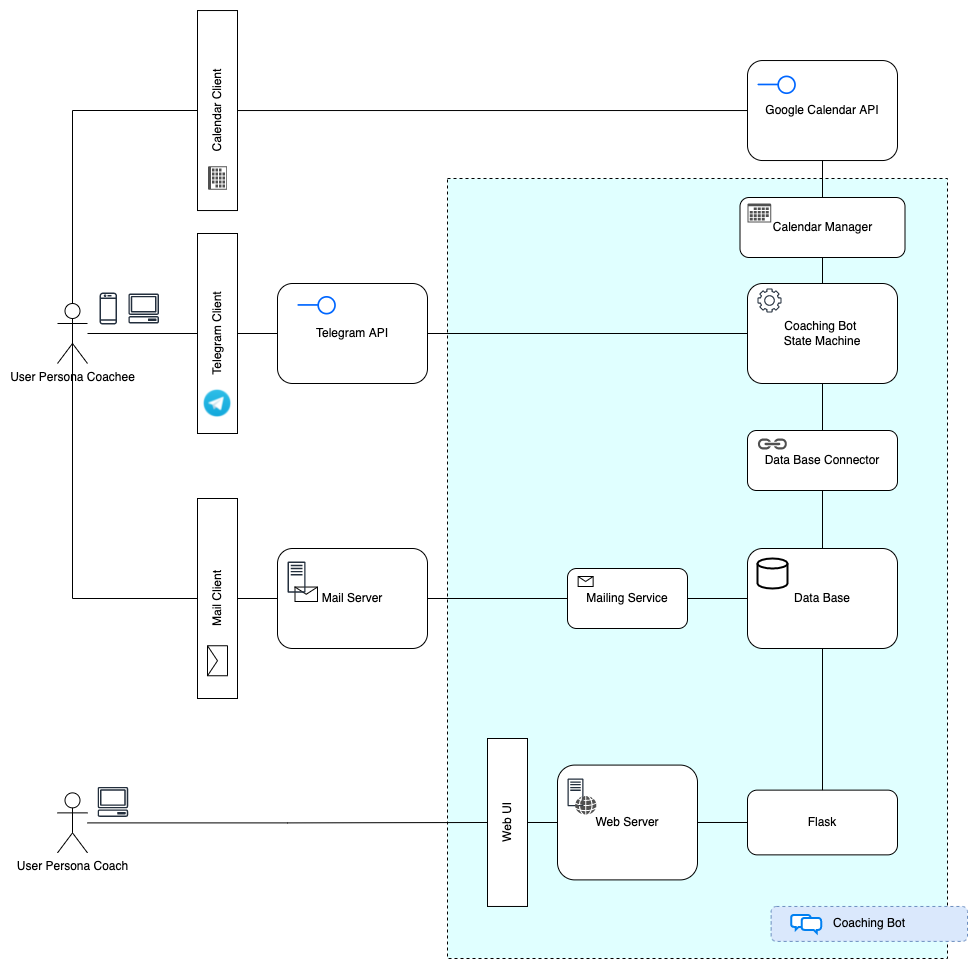
\includegraphics[width=1.0\textwidth]{images/220320_PA28464_Architecture.png}
		\caption{Konzeptionelle Architektur für das Projekt \emph{Der Coaching Bot}}
		\label{fig: architecture}
	\end{figure}

	Wie in Abbildung \ref{fig: architecture} skizziert, besteht der Kern des Bots auf einem endlichen Automaten (state machine), der Zustände vordefiniert und festlegt, wann sich welcher Nutzer in welchem Zustand befindet und von welchem in welchen Zustand er sich bewegen darf. An diesen Kern bindet sind als zentrales Steuerungselement des Bots alle anderen Systeme angebunden. Dazu gehören:
	\begin{enumerate}
		\item Die Datenbank zur Speicherung der Nutzerdaten
		\item Die Telegram API, über die die Kommunikation mit dem Telegram Client abgewickelt wird
		\item Die Google Calendar API, über die Events erstellt und versendet werden können
		\item Den Mail Server, über den E-Mails an den nutzer versendet werden können.
	\end{enumerate} 

	Der Nutzer interagiert mit dem ganzen System durch vier Kanäle - hier links ersichtlich:
	\begin{enumerate}
		\item Telegram Client: Kommunikation mit dem Bot
		\item Calendar Client: Erhalt, Annahme sowie Ablehnung der vereinbarten Termine
		\item Mail Client: Erhalten der Zusammenfassung und Bestätigung
		\item Web Browser: Übersicht über Anmeldungen und Terminkalender
	\end{enumerate}

	Der Bot wird von Benutzern (links oben) via einem der verfügbaren Telegram Clients angesprochen und reagiert auf die Eingabe entsprechend. So können verschieden Funktionen ausgelöst werden. Bspw. werden Antworten zurückgegeben, Informationen gespeichert oder es wird ein Vorschlag gemacht und an den Nutzer zurückgegeben. Der Bot soll mit mehreren Benutzern gleichzeitig sprechen können. Das wird ermöglicht, weil alle Reaktionen des Bots mit der Kennung des jeweiligen Nutzers verknüpft sind. So spricht der Bot den Nutzer mit Namen an oder kann sich daran erinnnern, welche Fragen schon beantwortet wurden und welche nicht. \\ \\

	Daneben gibt es einen zweite, sehr einfache Web-Applikation, die auf Flask basiert und eine Web-GUI zur Verfügung stellt, über die die gesammelten Informationen dargestellt werden können. So kann ein Coach (links unten) sich, nachdem Bewerber den Prozess beendet haben, alle gesammelten Informationen sowie vereinbarte Termine in einer einfachen Web-GUI ansehen.

\section{Zustände \& Konversationsfluss}

	Im folgenden Zustandsdiagramm ist der Konversationsfluss des Bots auf hohem Abstraktionsniveau, nämlich als endlicher Automat (state machine) abgebildet. Es wird deutlich, dass der Bot einem einfachen Skript folgt und komplizierte Loops vermieden werden. 
	\begin{figure} %[hbtp]
		\centering
		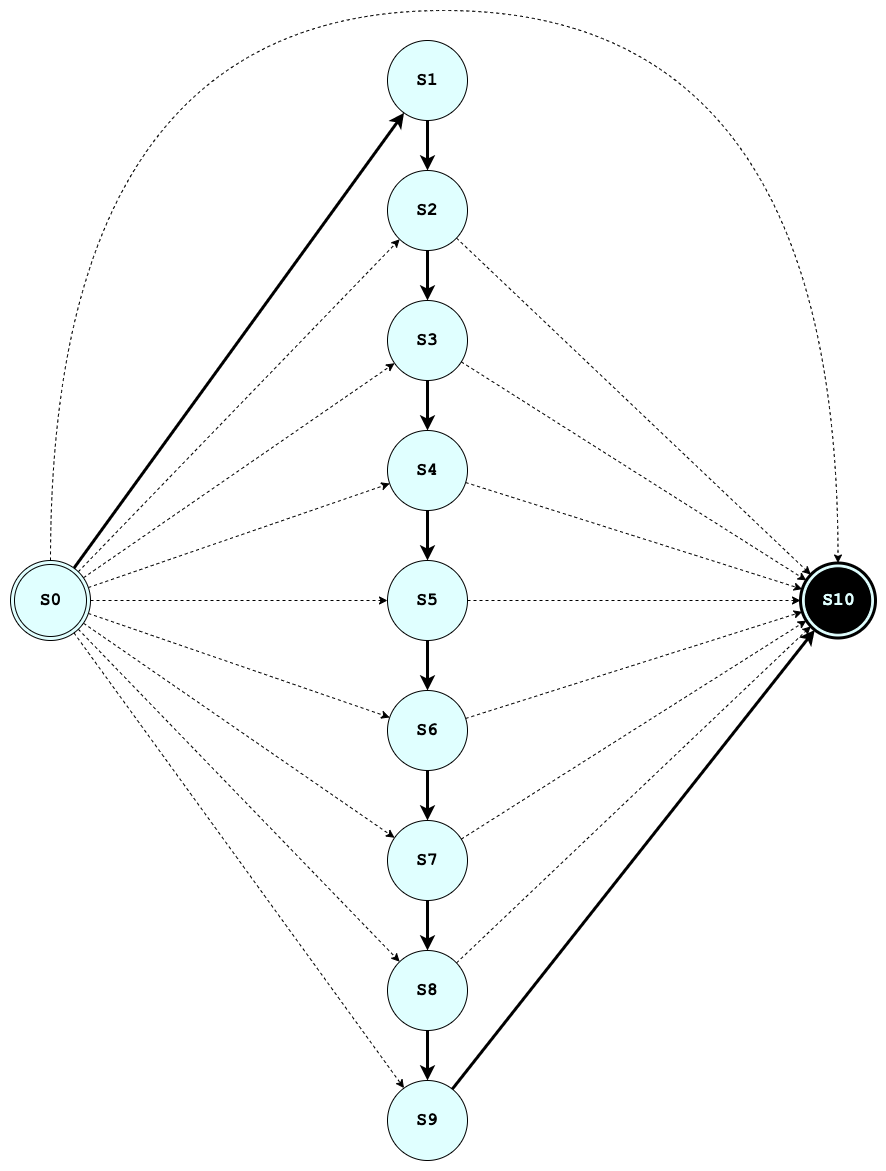
\includegraphics[width=1.0\textwidth]{images/220320_PA28464_State-Machine.png}
		\caption{Endlicher Automat des Konversationsflusses des Bots}
		\label{fig: state machine}
	\end{figure}

	Zustände:
	\begin{table} %[hbtp]
		\centering
		\begin{tabular}{l | l l l l}
			\textbf{Zustände} 	& \textbf{Beschreibung}\\
			\hline
			S0 					&		 START 			&		 Start: Applikation gestartet\\
			S1 					&		 BIO 			&		 Eingabemöglichkeit Biographie\\
			S2 					&		 GENDER 		&		 Eingabemöglichkeit Geschlecht\\
			S3 					&		 BIRTHDATE 		&		 Eingabemöglichkeit Geburtsdatum\\
			S4 					&		 EMAIL 			&		 Eingabemöglichkeit E-Mail Adresse\\
			S5 					&		 TELEPHONE 		&		 Eingabemöglichkeit Telefonnummer\\
			S6 					&		 LOCATION 		&		 Eingabemöglichkeit Ort\\
			S7 					&		 PHOTO 			&		 Eingabemöglichkeit Bild\\
			S8 					&		 SUMMARY 		&		 Zusammenfassung Daten\\
			S9 					&		 APPOINTMENT	&		 Terminvereinbarung \\
			S10 				&		 ENDE 			&		 Ende: Applikation beendet\\

		\end{tabular}
		\caption{Zustände des Konversationsflusses}
		\label{tab: states}
	\end{table}

	Der Haupt-Pfad ist hier fett eingezeichnet. Nebem diesem ist es aber auch möglich, dass der Nutzer nach einiger Zeit zum Bot zurück kommt und gerne an der Stelle weitermachen würde, wo er aufgehört hat. In diesem Fall, dient der Zustand \verb|S0| (START) als zentraler Einstiegspunkt. Hier wird analysiert, ob der Nutzer schon bekannt ist und falls ja, bis wohin er den Prozess bereits durchlaufen hat. Dann wird er dorthin weitergeleitet. Daher ist es möglich von START zu allen anderen Zuständen zu kommen, auch wenn das nicht die Regel ist. Hat der Nutzer den Prozess bereits abgeschlossen, so kann er sogar von S0 direkt in S10 (ENDE) landen und wird entsprechend benachrichtigt. Da dem Nutzer die Möglichkeit gegeben werden soll, den Prozess jederzeit zu beenden, ist es auch möglich, von jedem Zustand in \verb|S10| (ENDE) zu gelangen.\footnote{Der Konversationsfluss ist in einer sehr detaillierteren Ansicht verfügbar, in der der Unterschied zwischen dem hohen Abstraktionsniveau des Automaten und der Realität sichtbar wird. So lässt sich leicht erkennen, wo die Konversation beginnt und welche Zustände und Übergänge möglich sind: \url{https://github.com/mwel/coaching_bot/blob/main/thesis/images/220320_PA28464_Conversation_Flow.svg}} 